% This is "sig-alternate.tex" V2.0 May 2012
% This file should be compiled with V2.5 of "sig-alternate.cls" May 2012
%
% This example file demonstrates the use of the 'sig-alternate.cls'
% V2.5 LaTeX2e document class file. It is for those submitting
% articles to ACM Conference Proceedings WHO DO NOT WISH TO
% STRICTLY ADHERE TO THE SIGS (PUBS-BOARD-ENDORSED) STYLE.
% The 'sig-alternate.cls' file will produce a similar-looking,
% albeit, 'tighter' paper resulting in, invariably, fewer pages.
%
% ----------------------------------------------------------------------------------------------------------------
% This .tex file (and associated .cls V2.5) produces:
%       1) The Permission Statement
%       2) The Conference (location) Info information
%       3) The Copyright Line with ACM data
%       4) NO page numbers
%
% as against the acm_proc_article-sp.cls file which
% DOES NOT produce 1) thru' 3) above.
%
% Using 'sig-alternate.cls' you have control, however, from within
% the source .tex file, over both the CopyrightYear
% (defaulted to 200X) and the ACM Copyright Data
% (defaulted to X-XXXXX-XX-X/XX/XX).
% e.g.
% \CopyrightYear{2007} will cause 2007 to appear in the copyright line.
% \crdata{0-12345-67-8/90/12} will cause 0-12345-67-8/90/12 to appear in the copyright line.
%
% ---------------------------------------------------------------------------------------------------------------
% This .tex source is an example which *does* use
% the .bib file (from which the .bbl file % is produced).
% REMEMBER HOWEVER: After having produced the .bbl file,
% and prior to final submission, you *NEED* to 'insert'
% your .bbl file into your source .tex file so as to provide
% ONE 'self-contained' source file.
%
% ================= IF YOU HAVE QUESTIONS =======================
% Questions regarding the SIGS styles, SIGS policies and
% procedures, Conferences etc. should be sent to
% Adrienne Griscti (griscti@acm.org)
%
% Technical questions _only_ to
% Gerald Murray (murray@hq.acm.org)
% ===============================================================
%
% For tracking purposes - this is V2.0 - May 2012

\documentclass{acm_proc_article-me}

\begin{document}
%
% --- Author Metadata here ---
%\conferenceinfo{WOODSTOCK}{'97 El Paso, Texas USA}
%\CopyrightYear{2007} % Allows default copyright year (20XX) to be over-ridden - IF NEED BE.
%\crdata{0-12345-67-8/90/01}  % Allows default copyright data (0-89791-88-6/97/05) to be over-ridden - IF NEED BE.
% --- End of Author Metadata ---

\title{Multimodal Person Discovery in Broadcast TV}
%
% You need the command \numberofauthors to handle the 'placement
% and alignment' of the authors beneath the title.
%
% For aesthetic reasons, we recommend 'three authors at a time'
% i.e. three 'name/affiliation blocks' be placed beneath the title.
%
% NOTE: You are NOT restricted in how many 'rows' of
% "name/affiliations" may appear. We just ask that you restrict
% the number of 'columns' to three.
%
% Because of the available 'opening page real-estate'
% we ask you to refrain from putting more than six authors
% (two rows with three columns) beneath the article title.
% More than six makes the first-page appear very cluttered indeed.
%
% Use the \alignauthor commands to handle the names
% and affiliations for an 'aesthetic maximum' of six authors.
% Add names, affiliations, addresses for
% the seventh etc. author(s) as the argument for the
% \additionalauthors command.
% These 'additional authors' will be output/set for you
% without further effort on your part as the last section in
% the body of your article BEFORE References or any Appendices.

\numberofauthors{3} 

\author{
% You can go ahead and credit any number of authors here,
% e.g. one 'row of three' or two rows (consisting of one row of three
% and a second row of one, two or three).
%
% The command \alignauthor (no curly braces needed) should
% precede each author name, affiliation/snail-mail address and
% e-mail address. Additionally, tag each line of
% affiliation/address with \affaddr, and tag the
% e-mail address with \email.
%
% 1st. author
\alignauthor
Johann Poignant\\
\alignauthor
Herv\'e Bredin\\
       \affaddr{LIMSI - CNRS - Rue John Von Neumann, Orsay, France.}
       \email{firstname.lastname@limsi.fr}
\alignauthor
Claude Barras\\
}
% There's nothing stopping you putting the seventh, eighth, etc.
% author on the opening page (as the 'third row') but we ask,
% for aesthetic reasons that you place these 'additional authors'
% in the \additional authors block, viz.
\date{30 July 2015}
% Just remember to make sure that the TOTAL number of authors
% is the number that will appear on the first page PLUS the
% number that will appear in the \additionalauthors section.

\maketitle
\begin{abstract}
Given raw TV broadcasts, each shot must be automatically tagged with the name(s) of people who can be both seen as well as heard in the shot. The list of people is not known a priori and their names must be discovered in an unsupervised way from provided text overlay or speech transcripts. The task will be evaluated on a new French corpus (provided by INA), using standard information retrieval metrics based on a posteriori collaborative annotation of the corpus.
\end{abstract}

\section{Motivation}

TV archives maintained by national institutions such as the French INA, the Netherlands Institute for Sound \& Vision, or the BBC are rapidly growing in size. The need for applications that make these archives searchable has led researchers to devote concerted effort to developing technologies that create indexes.

Indexes that represent the location and identity of people in the archive are indispensable for searching archives. Human nature leads people to be very interested in other people. However, at the moment that content is created or broadcast, it is not always possible to predict which people will be the most important to find in the future. Someone who appeared in a broadcast, but was relatively unnoticed, might suddenly start generating a buzz and become a trending topic on social networks or search engines. For this reason, it is not possible to assume that a biometric models capable of detecting an individual, will be present at indexing time. For some people such a model may not be available in advance, simply because they are not (yet) famous. In such cases, it is also possible that archivists annotating content by hand do not even know the name of the person. The goal of this task is to address the challenge of indexing people in the archive, under real-world conditions (i.e., there is no pre-set list of people to index). 

This task represents an extension of the (now completed) French REPERE challenge, which focused on multimodal person recognition in TV broadcast. The main objective of this challenge was to answer the two questions "Who speaks when?" and "Who appears when?" using any sources of information (including pre-existing biometric models and person names extracted from text overlay and speech transcripts). In this new task, only unsupervised algorithms (i.e., algorithms not relying on pre-existing labels or biometric models) are admitted. To ensure high quality indexes, those algorithms should also help human annotators double-check these indexes by providing an evidence of the claimed identity (especially for people who are not yet famous).

\begin{figure*}[t]
 \center 
 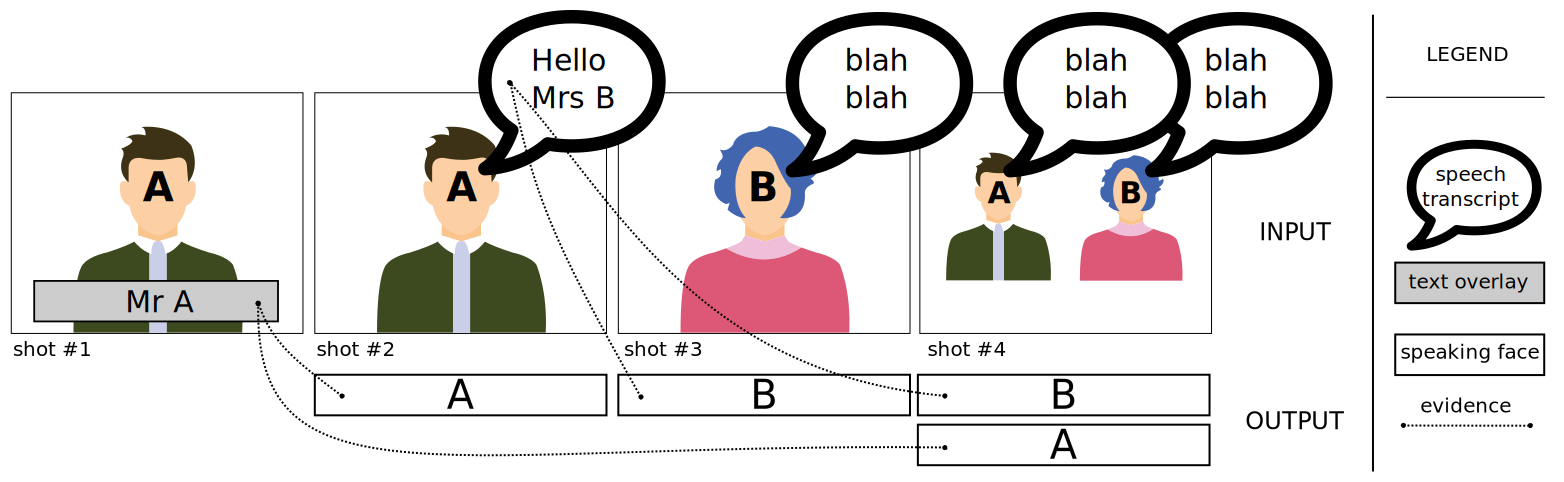
\includegraphics[width=0.7\linewidth]{figs/evidence.png}
 \centering
 \caption {What is an evidence of the person identities}
 \label{fig:evidence}
\end{figure*}

\section{Goal of the task}

Given raw TV broadcasts, each shot must be automatically tagged with the name(s) of people who can be both seen as well as heard in the shot. The list of people is not known a priori and their names must be discovered in an unsupervised way from provided text overlay or speech transcripts. 

Participants are provided with a collection of TV broadcasts pre-segmented into shots, along with the output of several baseline components: speaker diarization, face detection and tracking, speech transcription, video OCR and named entity detection. 

Participants are asked to provide, for each shot, the list of names of persons speaking AND appearing at the same time. The main novelty of the task is that the list of persons is not provided a priori, and person models (neither voice nor face) may not be trained on external data. The only way to identify a person is by finding their name in the audio (e.g., using speech transcription) or visual (e.g., using optical character recognition) streams and associating them to the correct person making the task completely unsupervised. For each returned shot, participants are also asked to provide the evidence justifying their assertion (e.g. a short excerpt of the test set showing the person AND its name at the same time).



The goal of the task (what the participants had to do)

\section{Related works}

Related work (papers that are particularly important for the task)

REPERE task


\section{The data set}

The original REPERE corpus set will be used as development set. This corpus is composed of various TV shows (focusing on news, politics and people) from two French TV channels. It will be distributed by ELDA (Evaluation and Language resources Distribution Agency) freely or at distribution cost. Among those 137 hours, 50 are already manually annotated. Audio annotations are dense and provide speech transcripts and identity-labeled speech turns. Video annotations are sparse (one image every 10 seconds) and provide overlaid text transcripts and identity-labeled face segmentation. Both speech and overlaid text transcripts are tagged with named entities.

The test set is composed of two corpora, a French TV news corpus provided by INA and the Catalan AGORA corpus. The INA corpus contains 115 hours of video, corresponding to 181 editions of evening broadcast news "Le 20 heures" of French public channel "France 2", from January 1st 2007 to June 30st 2007. Videos are provided as 181 MPEG1 files.


\section{Ground truth}

Here is how the search experiment is designed. Based on participant submissions, we will select a set of queries following the form: “PersonFirstName PersonLastName” possibly restricted to a temporal interval. For each query and for each video within the chosen period, the shots for which a submitted person name is close to the query name (i.e. by applying a predefined threshold on a string distance) will be selected and ranked according to their confidence score.

\subsection{Collaborative annotation}

Groundtruth will be created a posteriori by manually checking the top N shots proposed by participants for each request and the associated evidence. We will kindly ask participants to contribute to the annotation via the collaborative annotation webapp developed in the framework of the CHISTERA Camomile project. Evidences provided by participants will ease and speed up the annotation process. An online adjudication interface will be opened after the first round of evaluations to solve remaining ambiguous cases.

\subsection{Web interface}

\section{Evaluation procedure}

This procedure results in an Average Precision specific to the query and to the video. In order to prevent giving too much weight to predominant people or to individual video, we will first compute the Mean Average Precision over all videos where a particular person is detected, and then compute a Mean Mean Average Precision over all persons.

Average Precision will be modified slightly to take the quality of the evidence into account. Hence, instead of a binary judgment (relevant vs. not relevant), shot relevance will be computed as follows (the value of α will be discussed during the development phase):

{shot relevance} = α . {shot is relevant} + (1 - α) . {evidence is correct}



\section{Baseline}

\subsection{Late naming}

Propagation of written names onto speaker cluster. 

Propagation of speaker identities to the face with the higher probability to be the speaker

\subsection{Constraint clustering}



\section{Acknowledgments}

INA \\
ELDA \\


% The following two commands are all you need in the
% initial runs of your .tex file to
% produce the bibliography for the citations in your paper.
\bibliographystyle{abbrv}
\bibliography{publi}  % sigproc.bib is the name of the Bibliography in this case
% You must have a proper ".bib" file
%  and remember to run:
% latex bibtex latex latex
% to resolve all references


\end{document}
